\ifx\wholebook\relax\else

% --------------------------------------------
% Lulu:

    \documentclass[a4paper,12pt,twoside]{../includes/ThesisStyle}

	\usepackage[T1]{fontenc} %%%key to get copy and paste for the code!
%\usepackage[utf8]{inputenc} %%% to support copy and paste with accents for frnehc stuff
\usepackage{times}
\usepackage{ifthen}
\usepackage{xspace}
\usepackage{alltt}
\usepackage{latexsym}
\usepackage{url}            
\usepackage{amssymb}
\usepackage{amsfonts}
\usepackage{amsmath}
\usepackage{stmaryrd}
\usepackage{enumerate}
\usepackage{cite}
%\usepackage[pdftex,colorlinks=true,pdfstartview=FitV,linkcolor=blue,citecolor=blue,urlcolor=blue]{hyperref}
\usepackage{xspace}
%\usepackage{graphicx}
\usepackage{subfigure}
\usepackage[scaled=0.85]{helvet}
        
        
\newcommand{\sepe}{\mbox{>>}}
\newcommand{\pack}[1]{\emph{#1}}
\newcommand{\ozo}{\textsc{oZone}\xspace}
\newcommand\currentissues{\par\smallskip\textbf{Current Issues -- }}

\newboolean{showcomments}
\setboolean{showcomments}{true}
\ifthenelse{\boolean{showcomments}}
  {\newcommand{\bnote}[2]{
	\fbox{\bfseries\sffamily\scriptsize#1}
    {\sf\small$\blacktriangleright$\textit{#2}$\blacktriangleleft$}
    % \marginpar{\fbox{\bfseries\sffamily#1}}
   }
   \newcommand{\cvsversion}{\emph{\scriptsize$-$Id: macros.tex,v 1.1.1.1 2007/02/28 13:43:36 bergel Exp $-$}}
  }
  {\newcommand{\bnote}[2]{}
   \newcommand{\cvsversion}{}
  } 


\newcommand{\here}{\bnote{***}{CONTINUE HERE}}
\newcommand{\nb}[1]{\bnote{NB}{#1}}
\newcommand{\fix}[1]{\bnote{FIX}{#1}}
%%%% add your own macros 

\newcommand{\sd}[1]{\bnote{Stef}{#1}}
\newcommand{\ja}[1]{\bnote{Jannik}{#1}}
\newcommand{\na}[1]{\bnote{Nico}{#1}}
%%% 


\newcommand{\figref}[1]{Figure~\ref{fig:#1}}
\newcommand{\figlabel}[1]{\label{fig:#1}}
\newcommand{\tabref}[1]{Table~\ref{tab:#1}}
\newcommand{\layout}[1]{#1}
\newcommand{\commented}[1]{}
\newcommand{\secref}[1]{Section \ref{sec:#1}}
\newcommand{\seclabel}[1]{\label{sec:#1}}

%\newcommand{\ct}[1]{\textsf{#1}}
\newcommand{\stCode}[1]{\textsf{#1}}
\newcommand{\stMethod}[1]{\textsf{#1}}
\newcommand{\sep}{\texttt{>>}\xspace}
\newcommand{\stAssoc}{\texttt{->}\xspace}

\newcommand{\stBar}{$\mid$}
\newcommand{\stSelector}{$\gg$}
\newcommand{\ret}{\^{}}
\newcommand{\msup}{$>$}
%\newcommand{\ret}{$\uparrow$\xspace}

\newcommand{\myparagraph}[1]{\noindent\textbf{#1.}}
\newcommand{\eg}{\emph{e.g.,}\xspace}
\newcommand{\ie}{\emph{i.e.,}\xspace}
\newcommand{\ct}[1]{{\textsf{#1}}\xspace}


\newenvironment{code}
    {\begin{alltt}\sffamily}
    {\end{alltt}\normalsize}

\newcommand{\defaultScale}{0.55}
\newcommand{\pic}[3]{
   \begin{figure}[h]
   \begin{center}
   \includegraphics[scale=\defaultScale]{#1}
   \caption{#2}
   \label{#3}
   \end{center}
   \end{figure}
}

\newcommand{\twocolumnpic}[3]{
   \begin{figure*}[!ht]
   \begin{center}
   \includegraphics[scale=\defaultScale]{#1}
   \caption{#2}
   \label{#3}
   \end{center}
   \end{figure*}}

\newcommand{\infe}{$<$}
\newcommand{\supe}{$\rightarrow$\xspace}
\newcommand{\di}{$\gg$\xspace}
\newcommand{\adhoc}{\textit{ad-hoc}\xspace}

\usepackage{url}            
\makeatletter
\def\url@leostyle{%
  \@ifundefined{selectfont}{\def\UrlFont{\sf}}{\def\UrlFont{\small\sffamily}}}
\makeatother
% Now actually use the newly defined style.
\urlstyle{leo}



	\usepackage{amsmath,amssymb}             % AMS Math
% \usepackage[french]{babel}
\usepackage[latin1]{inputenc}
\usepackage[T1]{fontenc}
\usepackage[left=1.5in,right=1.3in,top=1.1in,bottom=1.1in,includefoot,includehead,headheight=13.6pt]{geometry}
\renewcommand{\baselinestretch}{1.05}

\usepackage{multicol}

% Table of contents for each chapter

\usepackage[nottoc, notlof, notlot]{tocbibind}
\usepackage{minitoc}
\setcounter{minitocdepth}{1}
\mtcindent=15pt
% Use \minitoc where to put a table of contents

\usepackage{enumitem}

\usepackage{aecompl}

% Glossary / list of abbreviations

%\usepackage[intoc]{nomencl}
%\renewcommand{\nomname}{List of Abbreviations}
%
%\makenomenclature

% My pdf code

\usepackage[pdftex]{graphicx}
\usepackage[a4paper,pagebackref,hyperindex=true]{hyperref}

\usepackage{pgfplotstable,booktabs,colortbl}
\pgfplotsset{compat=1.8}

% Links in pdf
\usepackage{color}
\definecolor{linkcol}{rgb}{0,0,0.4} 
\definecolor{citecol}{rgb}{0.5,0,0} 

% Change this to change the informations included in the pdf file

% See hyperref documentation for information on those parameters

\hypersetup
{
bookmarksopen=true,
pdftitle="Sista: a Metacircular Architecture for Runtime Optimisation Persistence",
pdfauthor="Clement BERA", 
pdfsubject="Thesis", %subject of the document
%pdftoolbar=false, % toolbar hidden
pdfmenubar=true, %menubar shown
pdfhighlight=/O, %effect of clicking on a link
colorlinks=true, %couleurs sur les liens hypertextes
pdfpagemode=None, %aucun mode de page
pdfpagelayout=SinglePage, %ouverture en simple page
pdffitwindow=true, %pages ouvertes entierement dans toute la fenetre
linkcolor=linkcol, %couleur des liens hypertextes internes
citecolor=citecol, %couleur des liens pour les citations
urlcolor=linkcol %couleur des liens pour les url
}

% definitions.
% -------------------

\setcounter{secnumdepth}{3}
\setcounter{tocdepth}{1}

% Some useful commands and shortcut for maths:  partial derivative and stuff

\newcommand{\pd}[2]{\frac{\partial #1}{\partial #2}}
\def\abs{\operatorname{abs}}
\def\argmax{\operatornamewithlimits{arg\,max}}
\def\argmin{\operatornamewithlimits{arg\,min}}
\def\diag{\operatorname{Diag}}
\newcommand{\eqRef}[1]{(\ref{#1})}

\usepackage{rotating}                    % Sideways of figures & tables
%\usepackage{bibunits}
%\usepackage[sectionbib]{chapterbib}          % Cross-reference package (Natural BiB)
%\usepackage{natbib}                  % Put References at the end of each chapter
                                         % Do not put 'sectionbib' option here.
                                         % Sectionbib option in 'natbib' will do.
\usepackage{fancyhdr}                    % Fancy Header and Footer

% \usepackage{txfonts}                     % Public Times New Roman text & math font
  
%%% Fancy Header %%%%%%%%%%%%%%%%%%%%%%%%%%%%%%%%%%%%%%%%%%%%%%%%%%%%%%%%%%%%%%%%%%
% Fancy Header Style Options

\pagestyle{fancy}                       % Sets fancy header and footer
\fancyfoot{}                            % Delete current footer settings

%\renewcommand{\chaptermark}[1]{         % Lower Case Chapter marker style
%  \markboth{\chaptername\ \thechapter.\ #1}}{}} %

%\renewcommand{\sectionmark}[1]{         % Lower case Section marker style
%  \markright{\thesection.\ #1}}         %

\fancyhead[LE,RO]{\bfseries\thepage}    % Page number (boldface) in left on even
% pages and right on odd pages
\fancyhead[RE]{\bfseries\nouppercase{\leftmark}}      % Chapter in the right on even pages
\fancyhead[LO]{\bfseries\nouppercase{\rightmark}}     % Section in the left on odd pages

\let\headruleORIG\headrule
\renewcommand{\headrule}{\color{black} \headruleORIG}
\renewcommand{\headrulewidth}{1.0pt}
\usepackage{colortbl}
\arrayrulecolor{black}

\fancypagestyle{plain}{
  \fancyhead{}
  \fancyfoot{}
  \renewcommand{\headrulewidth}{0pt}
}

\usepackage{algorithm}
\usepackage[noend]{algorithmic}

%%% Clear Header %%%%%%%%%%%%%%%%%%%%%%%%%%%%%%%%%%%%%%%%%%%%%%%%%%%%%%%%%%%%%%%%%%
% Clear Header Style on the Last Empty Odd pages
\makeatletter

\def\cleardoublepage{\clearpage\if@twoside \ifodd\c@page\else%
  \hbox{}%
  \thispagestyle{empty}%              % Empty header styles
  \newpage%
  \if@twocolumn\hbox{}\newpage\fi\fi\fi}

\makeatother
 
%%%%%%%%%%%%%%%%%%%%%%%%%%%%%%%%%%%%%%%%%%%%%%%%%%%%%%%%%%%%%%%%%%%%%%%%%%%%%%% 
% Prints your review date and 'Draft Version' (From Josullvn, CS, CMU)
\newcommand{\reviewtimetoday}[2]{\special{!userdict begin
    /bop-hook{gsave 20 710 translate 45 rotate 0.8 setgray
      /Times-Roman findfont 12 scalefont setfont 0 0   moveto (#1) show
      0 -12 moveto (#2) show grestore}def end}}
% You can turn on or off this option.
% \reviewtimetoday{\today}{Draft Version}
%%%%%%%%%%%%%%%%%%%%%%%%%%%%%%%%%%%%%%%%%%%%%%%%%%%%%%%%%%%%%%%%%%%%%%%%%%%%%%% 

\newenvironment{maxime}[1]
{
\vspace*{0cm}
\hfill
\begin{minipage}{0.5\textwidth}%
%\rule[0.5ex]{\textwidth}{0.1mm}\\%
\hrulefill $\:$ {\bf #1}\\
%\vspace*{-0.25cm}
\it 
}%
{%

\hrulefill
\vspace*{0.5cm}%
\end{minipage}
}

\let\minitocORIG\minitoc
\renewcommand{\minitoc}{\minitocORIG \vspace{1.5em}}

\usepackage{multirow}
\usepackage{slashbox}

\newenvironment{bulletList}%
{ \begin{list}%
	{$\bullet$}%
	{\setlength{\labelwidth}{25pt}%
	 \setlength{\leftmargin}{30pt}%
	 \setlength{\itemsep}{\parsep}}}%
{ \end{list} }

\newtheorem{definition}{D�finition}
\renewcommand{\epsilon}{\varepsilon}

% centered page environment

\newenvironment{vcenterpage}
{\newpage\vspace*{\fill}\thispagestyle{empty}\renewcommand{\headrulewidth}{0pt}}
{\vspace*{\fill}}



	\graphicspath{{.}{../figures/}}
	\begin{document}
\fi

\chapter{Future work}
\label{chap:futureWork}
\minitoc

This chapter discusses future work related to Sista. The focus is on research-oriented future work, but the first two sections also mention engineering-oriented future work (for instance, moving the architecture to production).

Section \ref{sec:archEvo} describes the evolution planned or considered for the overall architecture. Section \ref{sec:newOpt} discusses specifically the optimisations that could be implemented in the optimisation pipeline of Sista and which of them could be interesting research-wise. Section \ref{sec:useCase} details how the application of Sista on a real-world application requiring quick start-ups would be very valuable to support the thesis. Lastly, Section \ref{sec:energy} discusses briefly the potentially low energy consumption of the Sista VM and how it could be valuable in specific use-cases.

\section{Architecture evolution}
\label{sec:archEvo}

This section details the evolution of the Sista architecture that could be considered in the future. Section \ref{ss:FWInterface} describes the potential evolution of the interface VM-language: Sista is currently using an extended bytecode set to communicate between Scorch and Cogit, another representation may be more efficient. Section \ref{ss:FWIDE} explains the on-going work to integrate Sista with the development tools. The evaluation of the memory footprint required by Sista is precised in Section \ref{ss:FWMemFootprint}. Section \ref{ss:FWPlatDep} discusses the current platform-dependencies of the persistence of optimisations across start-ups and how these dependencies could be avoided. Section \ref{ss:FWProduct} briefly states the on-going work to move Sista to production.

\subsection{Interface VM-language}
\label{ss:FWInterface}

\paragraph{Stack-based or register-based IR.}The v-functions discussed in the thesis are currently encoded in a stack-based bytecode IR. This is somehow a problem as it is very difficult to implement an optimising compiler on a stack-based IR. For this reason, Scorch decompiles the v-function to a register-based IR (similar to TAC\footnote{Three Address Code}, but some operations such as virtual calls may have more than three parameters), performs the optimisations and translates it back to the stack-based bytecode. Cogit then takes the stack-based bytecode as input, and translates it to a register-based IR to generate the n-function. 

The stack-based extended bytecode sets has two main issues:
\begin{itemize}
	\item \textbf{Lack of information:} Scorch IR has significant information about the instructions (liveness, uses) than the stack-based bytecode. Information lost during the translation to the stack-based bytecode may be profitable for low-level optimization in Cogit.
	\item \textbf{Redondant conversion:} It feels a bit redondant, when compiling using Scorch then Cogit, to translate the register-based Scorch's IR to the stack-based bytecode representation only to translate it back to a register-based IR in Cogit as shown on Figure \ref{fig:FutureWorkRedondant}. We could consider encoding optimised v-functions in a register-based IR, to avoid those conversions.
\end{itemize}

\begin{figure}[h!]
    \begin{center}
        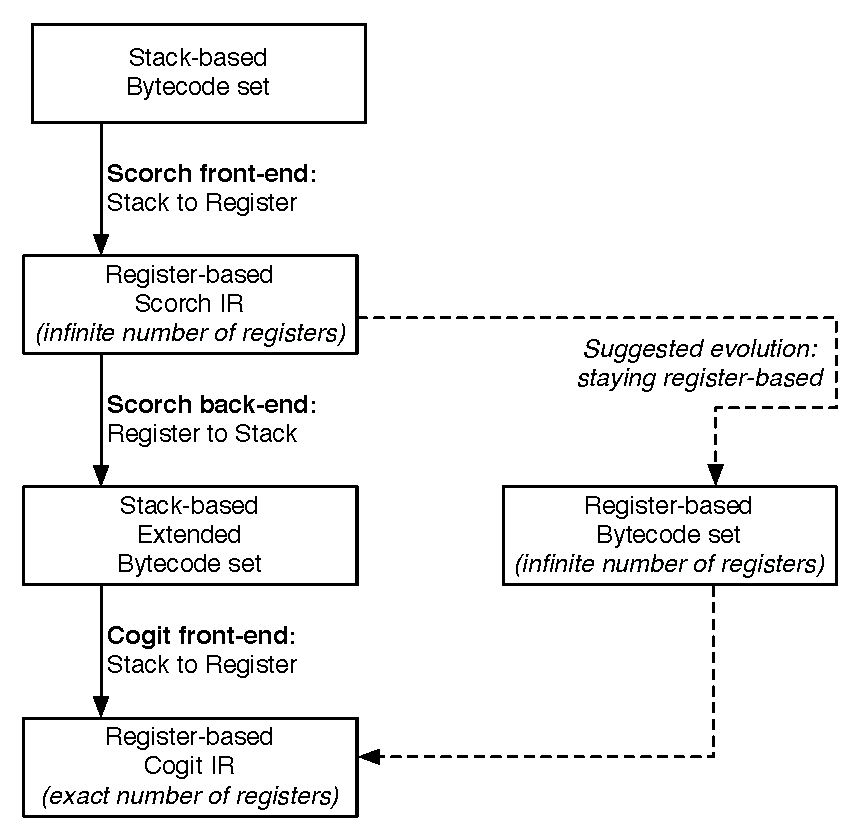
\includegraphics[width=0.4\linewidth]{FutureWorkRedondant}
        \caption{Redondant conversion}
        \label{fig:FutureWorkRedondant}
    \end{center}
\end{figure}

However, the extended bytecode set was designed stack-based for two main relevant reasons:
\begin{itemize}
	\item \textbf{Compatibility:} The existing bytecode set is stack-based, and having the extended bytecode set stack-based allows to generate optimised functions using both existing and new instructions. This was very convenient to have quickly a working version of Sista (only the new unsafe operations used needed to work to have the architecture working).
	\item \textbf{Machine-independent:} The alternative to a stack-based IR is usually a register-based IR. Scorch's IR can be seen as a register-based IR with an infinite number of registers, while Cogit's IR is a machine-specific register-based IR, with a fixed number of registers. The use of a stack-based IR allows to abstract away the extended bytecode set from machine-specific details, such as the exact number of registers. A register-based IR with an infinite number of registers also abstracts away from such low-level details, but it is not clear currently if a register-based IR with an infinite number of register is easier to actually translate to a machine-specific IR with a fixed number of register than a stack-based IR. Indeed, when the Javascript VM experts designed WebAssembly~\cite{WebAssembly}, they chose to use a stack-based IR over a register-based IR.
\end{itemize}	 

One future work is to design another extended bytecode set, register-based, and to evaluate the complexity of the representation in the back-end of Scorch and the front-end of Cogit.

\paragraph{Lower-level representation}

The extended bytecode set has instructions that are quite high-level, for example, accesses in an array. Such instructions generate multiple native instructions (the exact number of instructions depends on the memory representation of objects used and the processor used). As they are quite high-level, they abstract away from the memory representation of objects and the processor used. The extended bytecode set has, by design of the architecture, to be processor-independent but could be dependent on the memory representation of objects. This way, accesses to objects such are arrays could be represented in multiple instructions in Scorch instead of one, allowing potentially to fold new constants. The Cog VM features an abstract assembly instructions set, called Lowcode~\cite{Salg16a}, similar to WebAssembly~\cite{WebAssembly}. Scorch could target this representation instead of the current extended bytecode set. The future work is to implement such a back-end for Scorch and evaluate the complexity and the performance.

\subsection{Development tools integration}
\label{ss:FWIDE}

In Sista, we chose to implement Scorch as an unoptimised v-functions to optimised v-functions compiler in Smalltalk. Scorch is running in the same runtime as the application. This has different advantages, for example we could use all the Smalltalk development tools to implement and debug Scorch. However, there is a major draw-back. The language (in our case, Pharo) has now access to both the optimised and unoptimised stack frames. When the programmer now accesses the reification of a stack frame, depending on the optimisation state, an optimised frame might be shown. 

In some cases, for example when the programmer is working on Scorch itself, it is relevant to show in the development tools the optimised frames. In other cases, for example when the programmer is working in an end-user application on top of Pharo, development tools should show only unoptimised frames by transparently deoptimising stack frames.

We are now adapting the debugging tools to request deoptimise stack frames when needed. To do so, we are adding a development tool setting: one may or may not want to see the stack internals, depending on what one wants to implement.

\subsection{Memory footprint evaluation}
\label{ss:FWMemFootprint}

When implementing an optimising JIT, it is relevant to evaluate the memory footprint of the optimised code and the deoptimisation metadata. In our context, such an evaluation would be very interesting as:
\begin{itemize}
	\item Optimised functions are present both as v-functions and n-functions, potentially increasing the memory footprint.
	\item Deoptimisation metadata is split in two, one part in Cogit and one part in Scorch.
	\item As optimised v-functions are persisted across start-ups, it is interesting to know the size of the optimised v-functions and the corresponding deoptimisation metadata that is persisted.
\end{itemize}

Two future works are planned in this direction:
\begin{itemize}
	\item Does the split in the optimising induce more memory overhead than a classical function-based optimising JIT ?
	\item What is the size of the optimised v-functions and the corresponding deoptimisation metadata that is persisted across start-up ?
\end{itemize}

We did not evaluate the memory footprint because currently the deoptimisation metadata of Scorch is kept uncompressed. To compress it, we need to write, as part of the deoptimiser, a decompressor that is independent from the rest of the system. This requires a certain amount of engineering work that we did not have. We plan to work in the two directions in the near future.

\subsection{Platform-dependency}
\label{ss:FWPlatDep}

In Pharo, snapshots are independent of the processor and the OS used. It is proven as the same snapshot can be deployed on x86, ARMv6 and MIPSEL, as well as on Windows, Mac OS X, iOS, Linux, Android or RISC OS. However, the snapshots are dependent on the machine word size: 32 bit or 64 bit snapshots are not compatible. They are not compatible because the size of managed pointers is different, but also because the representation of specific objects, such as floating numbers, is different. It is however possible to convert offline a 32 bit snapshot to 64 bit and vice-versa. 

As some optimisations related to number arithmetics, such as overflow checks elimination, depends on the number representations, Scorch is currently dependent on the machine word size. A fully portable solution would either need not to do optimisations on machine word specific number representations or deoptimise the affected code on startup.

\subsection{Productisation}
\label{ss:FWProduct}

With the current version, the Sista VM is able to run all our benchmark suite. We are now able to do part of our development with the development tools, written in Smalltalk, running on the Sista VM. We still have work to do in the integration with the development tools, especially the debugger, but it seems that the biggest part of the work has been done. There are still some edge cases where the Sista VM is unstable, which still need to be fixed, but most code can be run on top of the Sista VM as it would be run on the production VM. We have started to integrate the dependencies of Sista in Pharo. We are now moving forward to integrate the optimiser in Pharo.

\section{New optimisations}
\label{sec:newOpt}

Another direction for future work is the implementation of new optimisations in Scorch or Cogit. 

\subsection{State-of-the-art optimisations}

The first thing to do is to implement all the state-of-the-art compiler optimisation in Scorch or Cogit, depending on the optimisation. Cogit features a naive register allocator, but we have plan to build a more advanced one and evaluate the performance difference. Scorch lacks multiple common optimisation passes, such as sparse conditional elimination, partial escape analysis and object allocation removal or floating-pointer related optimisations. Each of them could be implemented and the performance may then be measured.

\subsection{New optimisations}

Another direction would be to implement new optimisations that are not present in other compilers. One way to do so is to have new ideas on how to optimise code, or to design and implement new algorithms. This is far from trivial as many experts have worked in that direction in other compilers, but, hopefully, it is possible.

Alternatively, one could describe how traditional optimisations are implemented in the context of the split architecture we have in Sista. Which optimisation is implemented in Scorch, which one is implemented in Cogit, which one is implemented partly with both and requires some annotations in the optimised v-functions to communicate extra information from Scorch to Cogit. 

Lastly, the most interesting is likely to work on Smalltalk-specific optimisations that are not possible in other programming languages because other languages do not usually have specific features

Indeed, Smalltalk provides some unconventional operations that are not usually available in other object-oriented languages. These operations are problematic for the optimising JIT. The next paragraph provides some examples and discuss how such operations could be optimised.

\paragraph{Become.} One unconventional operation is called \emph{become}. It allows an object to swap identity with another one, \ie if an object \emph{a} becomes an object \emph{b}, all the references to \emph{a} now refer to \emph{b} and all the references to \emph{b} refer to \emph{a}. This operation was made efficient using different strategies described in \cite{Mir15a}. This feature has some implications in the context of an optimising JIT. At any interrupt point, there could be a green thread switch and from the other green thread, any of the temporary variable of the optimised stack frame could be changed to any object in the heap. This would invalidate all assumptions taken by Scorch.

\paragraph{Heavy stack manipulation.} The other unconventional operations are related to stack manipulation. Smalltalk reifies the call stack and allows the program not only to reflect on the call stack, but also to manipulate it. We discussed this in in Section \ref{par:frameToContext}, when we explained for example that the developer can set the caller of any stack frame to another frame.

\paragraph{Current Solution: Deoptimisation for unconventional operations.} All these operations are uncommon in a normal Smalltalk program at runtime.  They are usually used for implementing the debugging functionalities of Pharo. Currently, profiling production applications does not show that we would earn noticeable performance if we would optimise such cases. The solution therefore is to to always deoptimise the stack frames involved when such an operation happens. In the case of become, if a temporary variable in a stack frame executing an optimised method is edited, we deoptimise the frame. In the case of the stack manipulation, if the reification of the stack is mutated from the language, we deoptimise the corresponding mutated stack frames.

\paragraph{Future Work: Optimising unconventional operations.} It could be possible to have the runtime optimiser aware of these features and to handle them specifically. Especially, continuations and exceptions are built in Pharo in the language on top of the stack manipulation features. Optimising such features would allow to have efficient continuations and exceptions, in a similar way to the optimisation of exceptions described in \cite{Ogas01a}. 

\section{Application of Sista for quick start-ups}
\label{sec:useCase}

One point that is a bit unclear is how to use the Sista for quick start-up in a real-world application. Sure, it is possible to persist optimised functions across start-ups, but how are the optimised functions generated in the first place ? Are they generated from warm-up runs using a test suites or are they generated the first day the application is running and further day use the optimisations persisted from the first day ?

An example is the case of Azul~\cite{Azul}: a trading bank claims that they are able to use the optimised functions generated the day N-1 to improve the start-up performance of the day N. 

It seems that depending on the use-case where start-up performance matters (distributed application with short-lived slaves, such as the ones on Amazon lambda, Android application or Web pages), the solution is different. It would be very valuable to foxus on one of those use-cases and build a solid framework showing how to use the persistence of optimisations to reduce warm-up time and evaluate what is the cost for the application programmer (Does one have to do something specific to persist the optimisations or is it done automatically as part of a framework ?)

In the case of distributed application on Amazon lambda, slaves may live down to a couple seconds in case of a high-variant demand, so that there are very few slaves rent when the application is unused and a lot of slaves when the application is heavily used. Is it possible to build a fraework that automatically learn from the life of previous slaves what optimised functions are worth keeping, so when a new short-lived slaved is instantiated, it can reach peak performance very quickly ?

In the case of web pages, is it possible to build a global cache so all frequently used web pages would have pre-optimised code available from the runs of the previous users ?

All these applications of the persistence of optimisations across start-ups of Sista are very interesting and could be analysed in future work.

\section{Energy consumption evaluation}
\label{sec:energy}

Another interesting aspect in Sista is the energy saved at start-up by re-using persisted optimised functions instead of wasting cpu cycles re-generating them. 

The most relevant use-case is Android application. With the Dalvik VM or the Android Runtime, Google's team on the VM for Android application have switched multiple times their design from JIT compilation to AOT compilation then back to JIT compilation. The main problem is that JIT compilation yields better peak performance, but requires warm-up time for each application which wastes many cpu cycles, which corresponds in practice to an important part of the smart phone battery.

Sista would be relevant in this context as the application could be shipped unoptimised, but each time the user would use the application, the optimised functions generated would be persisted so further uses won't waste battery. This way, theoretically, the application could have very good peak performance due to the JIT while not wasting too many battery at start-up.

To work in this direction, one would need to evaluate the energy consumed by the VM to reach peak-performance. We did not work in this direction because we did not have expertise in enrgy consumption measurement, but this is definitely a relevant future work.

\section*{Conclusion}

This Chapter discussed the future works that may be done based on this Ph.D. The next Chapter summarises the contents of the thesis and concludes.

\ifx\wholebook\relax\else
    \end{document}
\fi